\section{Elektrisches und magnetisches Feld}
\begin{auf}
    480
\end{auf}
Ein Elektron tritt senkrecht zu den elektrischen Feldlinien mit der Geschwindigkeit $v_0$ in den Vakuumraum eines Plattenkondensators ein und durchläuft ihn auf gekrümmter
Bahn.
\begin{enumerate}
    \item[a] Um welche Art von Bahnkurve handelt es sich?
    \item[b] Der Kondensator habe einen Plattenabstand von $d=4cm$ und eine Plattenlänge von $l=10cm$, die an den Platten anliegende Spannung ist $U=300V$. Mit welcher Geschwindigkeit	$v$ tritt das Elektron aus dem Kondensatorfeld aus, wenn $v_0=1.6\cdot10^7\frac{m}{s}$?
    \item[c] Wie groß ist die Abweichung $h$ von der ursprünglichen Bewegungsrichtung beim Austritt aus dem Feld?
    \item[d] Welche Änderung der Gesamtenergie erfährt das Elektron beim Durchqueren des Feldes?	Ladung des Elektrons $e=1.602\cdot10^{-19}C$, Masse des Elektrons $m=9.109\cdot10^{-31}kg$.
\end{enumerate}
\begin{figure}[h]
    \centering
    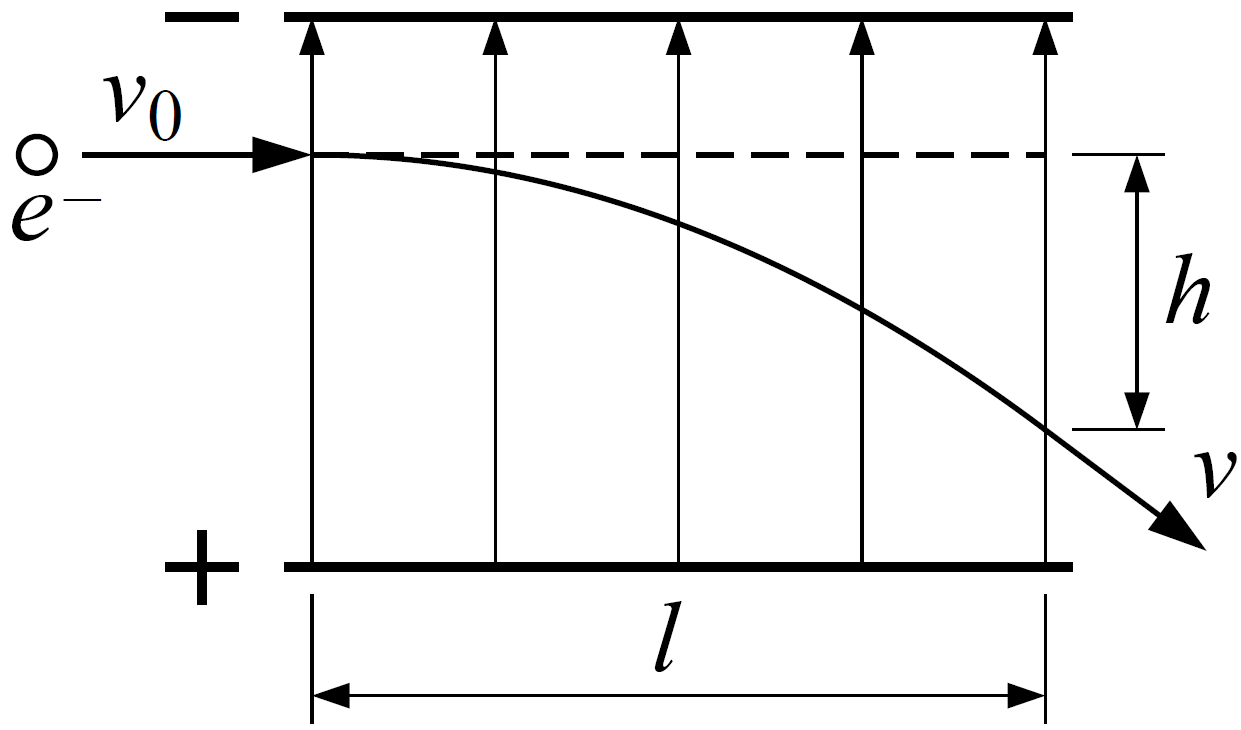
\includegraphics[width=0.7\linewidth]{images/480_0.png}
    \caption{Versuchsaufbau Aufgabe 480}
\end{figure}